% !TeX root = ../tesis.tex


\section{Secciones transversales}
\label{section:yth}

En la sección anterior se . En esta sección, se introducen las denominadas secciones transversales de extinción, absorción y esparcimiento, las cuales son cantidades macroscópicas medibles que proporcionan información sobre el sistema \cite{bohrenAbsorptionScatteringLight2008}. Para esto, se considera a la partícula embebida en un medio no absorbente e iluminada por una onda plana armónica en el tiempo. Teniendo en cuenta lo anterior, la energía transportada por los campos electromagnéticos y que es absorbida por la partícula $W_{abs}$, se calcula al integrar el promedio temporal del vector de Poynting\footnote{El promedio temporal del vector de Poynting es $\langle\vb{S}\rangle_t = (1/\tau)\int_t^{t+\tau}\vb{S}(t')dt'$, y para campos electromagnéticos del tipo ondas planas es $\langle\vb{S}\rangle_t = (1/2) \text{Re}[\vb{E} \times (\vb{B}/\mu)^{*}]$, donde $*$ denota la operación complejo conjugado \cite{bohrenAbsorptionScatteringLight2008}. } $\langle\vb{S}\rangle_t$  sobre una superficie cerrada $A$, que por simplificidad puede considerarse una esfera de radio $r$ mayor al de la partícula [ver Fig. \ref{WA}], es decir, 
\begin{tcolorbox}[ams align]
	W_{abs}=-\int_A \langle\vb{S}\rangle_t\cdot\vb{\hat{e}_r} \text{ dA},
	\label{flujopoynting}
\end{tcolorbox}
donde, debido a que $\langle\vb{S}\rangle_t$ y $\vb{\hat{e}_r}$ están orientados en la misma dirección, el signo negativo convierte a $W_{abs}$ en una cantidad positiva, de lo contrario, significaría que se genera energía dentro de la esfera \cite{bohrenAbsorptionScatteringLight2008}.
%
\begin{figure}[h]
	\centering
	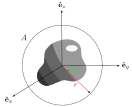
\includegraphics[width=6cm]{../../Figuras/WA.pdf}
	\caption{Esquema de la superficie de integración $A$ como una esfera de radio $r$ centrada en el origen y que contiene a la partícula de interés.}
	\label{WA}
\end{figure}
\\

\noindent Considerando la descomposición del vector de Poynting total en tres términos \cite{bohrenAbsorptionScatteringLight2008}
%
		
\begin{subequations}%
	\begin{tcolorbox}[
		ams align, breakable]
	\eqhalf{\langle\vb{S^i}\rangle_t=  \frac{1}{2}\:\mbox{Re}\{\vb{E}_i\times\vb{H}_i^*\},}%
	\eqhalf{\langle\vb{S^s}\rangle_t=  \frac{1}{2}\:\mbox{Re}\{\vb{E}_s\times\vb{H}_s^*\},}\\%
	\eqhalf{\langle\vb{S^{ext}}\rangle_t= \frac{1}{2}\:\mbox{Re}\{\vb{E}_i\times\vb{H}_s^*+\vb{E}_s\times\vb{H}_i^*\},}\label{eq:S}%
\end{tcolorbox}
\end{subequations}\vspace*{1em}
%

\noindent asociados al campo incidente, al campo esparcido y a la interacción entre los dos anteriores, respectivamente y donde Re$\{\cdot\}$ denota la parte real de un número complejo, se tiene que $W_{abs}=W_i-W_s+W_{ext}$, donde \cite{bohrenAbsorptionScatteringLight2008}
%
\begin{subequations} \label{eqs:W}
	\begin{tcolorbox}[
		ams align, breakable]
	W_i  &= -\int_{A}\langle\vb{S^i}\rangle_t\cdot\vb{\hat{e}_r}\text{ dA},\label{Wi}\\ W_s&=\int_{A}\langle\vb{S^s}\rangle_t\cdot\vb{\hat{e}_r}\text{ dA}, \label{Ws} \\ 
	W_{ext} &= -\int_{A}\langle\vb{S^{ext}}\rangle_t\cdot\vb{\hat{e}_r}\text{ dA},\label{Wext} 
	\end{tcolorbox}
\end{subequations}
%
cuyos signos están colocados de forma que sean cantidades positivas considerando las direcciones de los vectores de Poynting y de $\vb{\hat{e}_r}$. En particular, para un medio no absorbente, la energía que cruza la esfera es la misma que la que entra, por lo que $W_i$ se anula, entonces
%
\begin{equation}
	W_{ext}=W_{abs}+W_s.
\end{equation}
%%

Al considerar el campo incidente $\vb{E_i}=E\vb{\hat{e}_x}$ y a $\vb{H}_i=(1/\mu \omega)\: \vb{k} \times E \vb{\hat{e}_x}$ en un medio no absorbente, $W_a$ es independiente del radio $r$ de la superficie de integración, por lo que se puede considerar a $r$ lo suficientemente grande para estar en la región de campo lejano donde los campos se comportan como los generados por un dipolo inducido al iluminar un sistema de cargas y corrientes con un onda electromagnética de frecuencia angular $\omega$. Por lo cual, $W_{ext}$ está dado por \cite{bohrenAbsorptionScatteringLight2008}
%
\begin{equation*}
	W_{ext}=I_i\frac{4\pi}{k^2}\:\text{Re}\{(\vb{X}\cdot\vb{\hat{e}_x})_{\theta=0}\},
\end{equation*}
%
donde $\vb{X}$ es el vector de amplitud de esparcimiento dado por


y además, $I_i$ es la irradiancia de la onda incidente, que corresponde a la magnitud del vbtor de Poynting, y por consiguiente\footnote{Debido al teorema óptico, la extinción sólo depende de la amplitud de esparcimiento en la dirección de propagación y es el efecto combinado de la absorción en la partícula y el esparcimiento por la partícula en todas las direcciones \cite{bohrenAbsorptionScatteringLight2008}.},
%
\begin{equation}
	C_{ext}=\frac{W_{ext}}{I_i}=\frac{4\pi}{k^2}\:\text{Re}\{(\vb{X}\cdot\vb{\hat{e}_x})_{\theta=0}\}, \label{C_ext}
\end{equation}
%
que es la sección transversal de extinción y que posee dimensiones de área. La Ec. (\ref{C_ext}) puede ser reescrita como \cite{bohrenAbsorptionScatteringLight2008}
%
\begin{tcolorbox}[ams align]
	C_{ext}=C_{abs}+C_{sca}
	\label{C}
\end{tcolorbox}
%
donde $C_{abs}=W_{abs}/I_i$ y $C_{sca}=W_s/I_i$ corresponden a las secciones transversales de absorción y esparcimiento, respectivamente. Al sustituir las Ecs. (\ref{EH_s}) en la Ec. (\ref{Ws}) se obtiene
%
\begin{equation}
	C_{sca}=\int_0^{2\pi}\int_0^{\pi}\frac{|\vb{X}|^2}{k^2}\:\sin\theta\: \text{d}\theta\:\text{d}\phi.
	\label{C_sca_general}
\end{equation}
%%
Las Ecs. (\ref{C_ext})--(\ref{C_sca_general}) son propiedades macroscópicas y medibles, que proveen información sobre la energía absorbida y esparcida por una partícula.  \\

Al reescribir el vector de amplitud de esparcimiento [Ec. (\ref{Xvb})] en términos de la base vectorial esférica se obtiene \cite{bohrenAbsorptionScatteringLight2008}
%
\begin{equation}
	\vb{X}\cdot\vb{\hat{e}_x}=\frac{ik^3}{4\pi}\alpha(\sin^2\theta\cos^2\phi-1),  
	\label{X_esf}
\end{equation}
%
y sustituyendo la Ec. (\ref{X_esf}) en la Ec. (\ref{C_ext}), la sección transversal de extinción es
%
\begin{equation*}
	C_{ext}=k \mbox{Re}\left\{\left(i\alpha(\sin^2\theta\cos^2\phi-1)\right)_{\theta=0}\right\}=k\:\mbox{Re}\left\{-i\alpha\right\}=k\: \mbox{Im}\{\alpha\}.
\end{equation*}
%
Si el esparcimiento es despreciable con respecto a la absorción, la extinción corresponde a la absorción en mayor medida, tal que \cite{bohrenAbsorptionScatteringLight2008}
%
\begin{tcolorbox}[ams align]
	C_{abs}=k\: \mbox{Im}[\alpha].    
\end{tcolorbox}
Además, al sustituir la Ec. (\ref{Xvb}) en la Ec. (\ref{C_sca_general}), se obtiene \cite{bohrenAbsorptionScatteringLight2008}
%
\begin{tcolorbox}[ams align]
	C_{sca}=\frac{|\alpha|^2 k^2}{6\pi}.    
\end{tcolorbox}
